% Alternative evaluation plots; fig7 is an artifact-only diagnostic for Sec. 5.4.
% These captions and layouts are not the final manuscript versions.
% All four are full-width (figure*) and are drawn on a 16 in canvas with 20 pt text,
% so at \textwidth (7.0 in) the figure text prints at 8.75 pt.
% Values are checked by verify_sources.py; see README.md for regeneration commands.

\begin{figure*}[t]
  \centering
  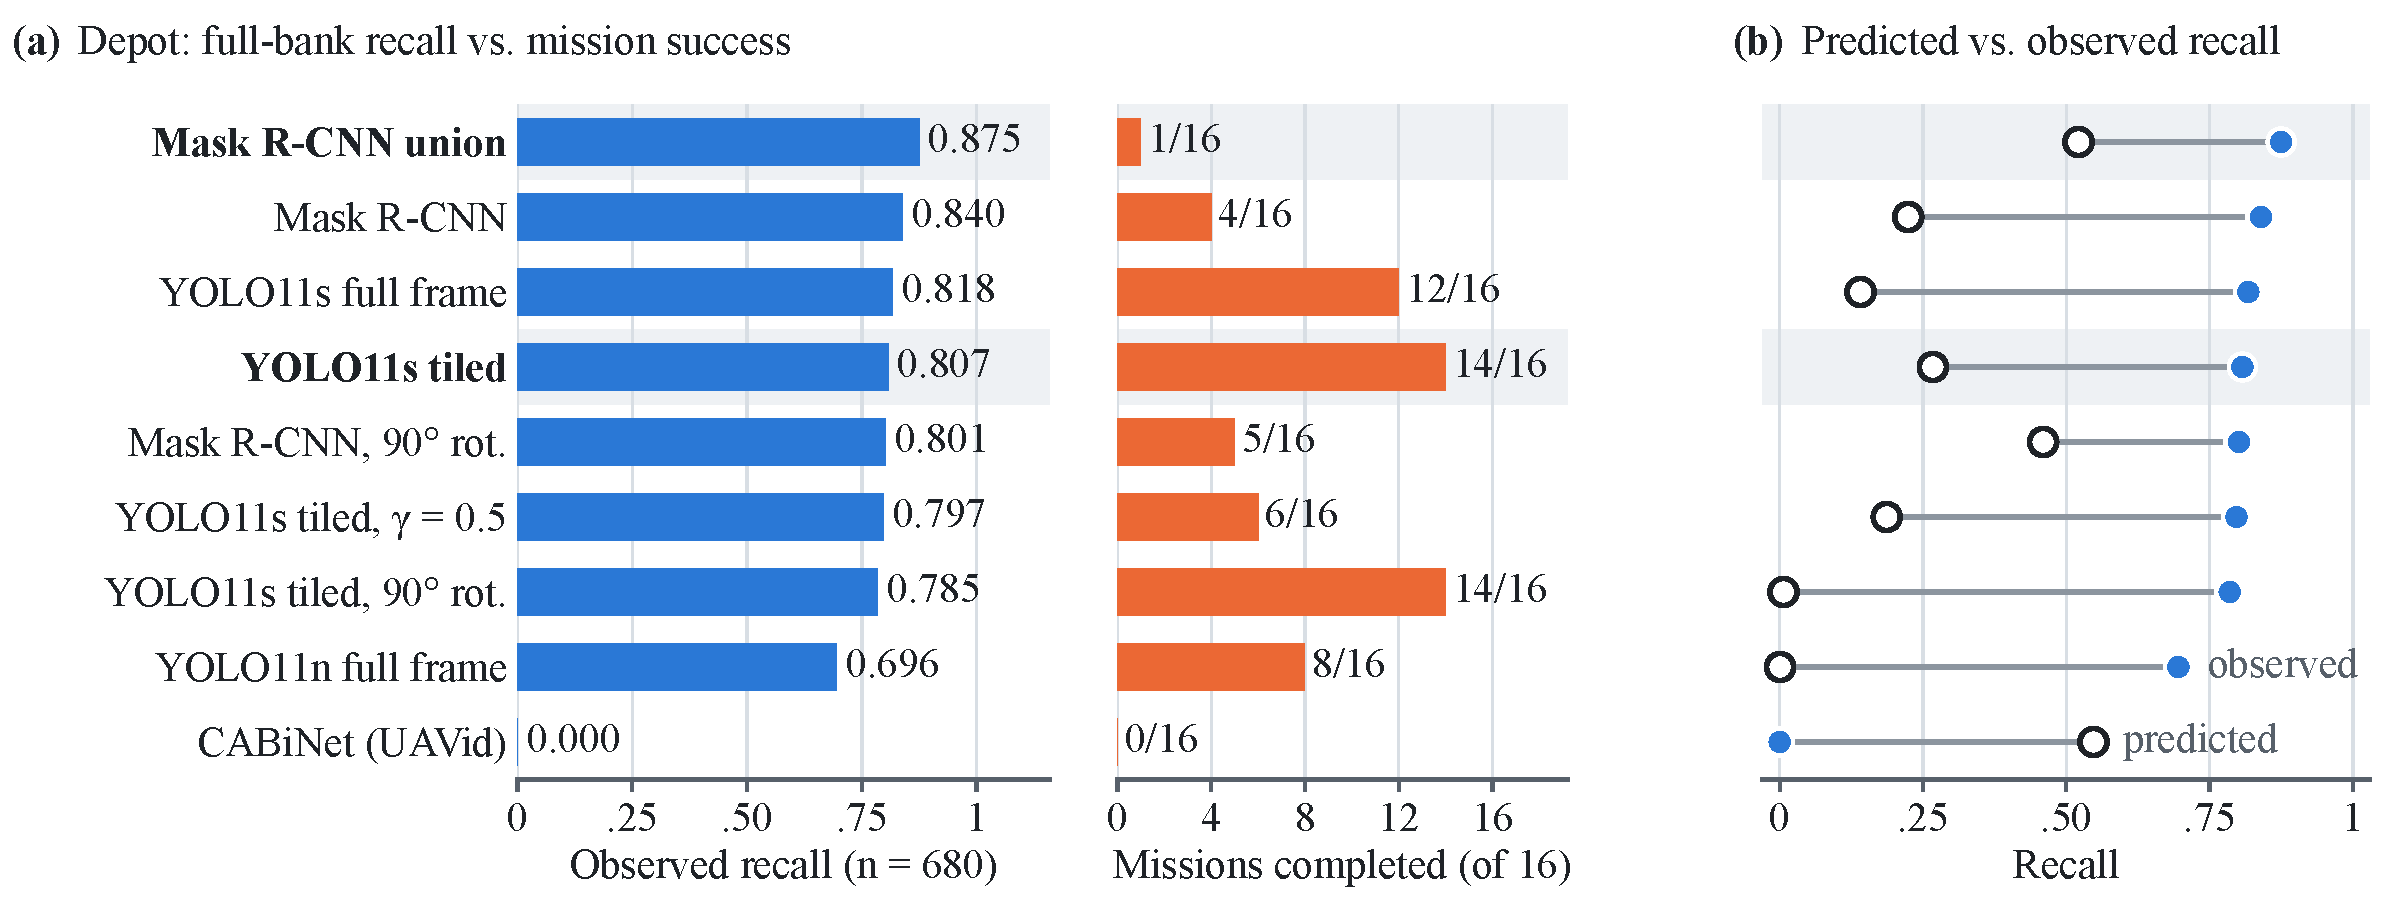
\includegraphics[width=\textwidth]{fig4}
  \caption{Perception accuracy versus mission fulfillment for all nine Depot perception
    configurations (multi-phase missions, 16 conditions). (a)~Full-bank observed target
    recall over 680 visible target observations in 240 captures, and missions completed by
    each configuration as a fixed policy. Mask R-CNN union has the highest recall (0.875)
    but completes 1/16 missions; tiled YOLO11s (0.807) completes 14/16. (b)~Recall
    predicted by the frozen quality estimator (hollow) versus observed recall (filled); the
    estimator was not refitted on Depot labels. Recall counts every potential capture,
    whereas a mission processes a latency-dependent subset of them, so this contrast does
    not isolate latency as the sole cause.}
  \Description{Nine perception configurations sorted by observed recall. Recall ranges
    from 0.875 for Mask R-CNN union to 0 for CABiNet, but missions completed do not follow
    recall: Mask R-CNN union completes 1 of 16 while tiled YOLO11s and rotated tiled YOLO11s
    complete 14 of 16. A second panel shows predicted recall far below observed recall for
    every configuration except CABiNet, which is predicted at 0.55 but observes 0.}
  \label{fig:perception-mission}
\end{figure*}

\begin{figure*}[t]
  \centering
  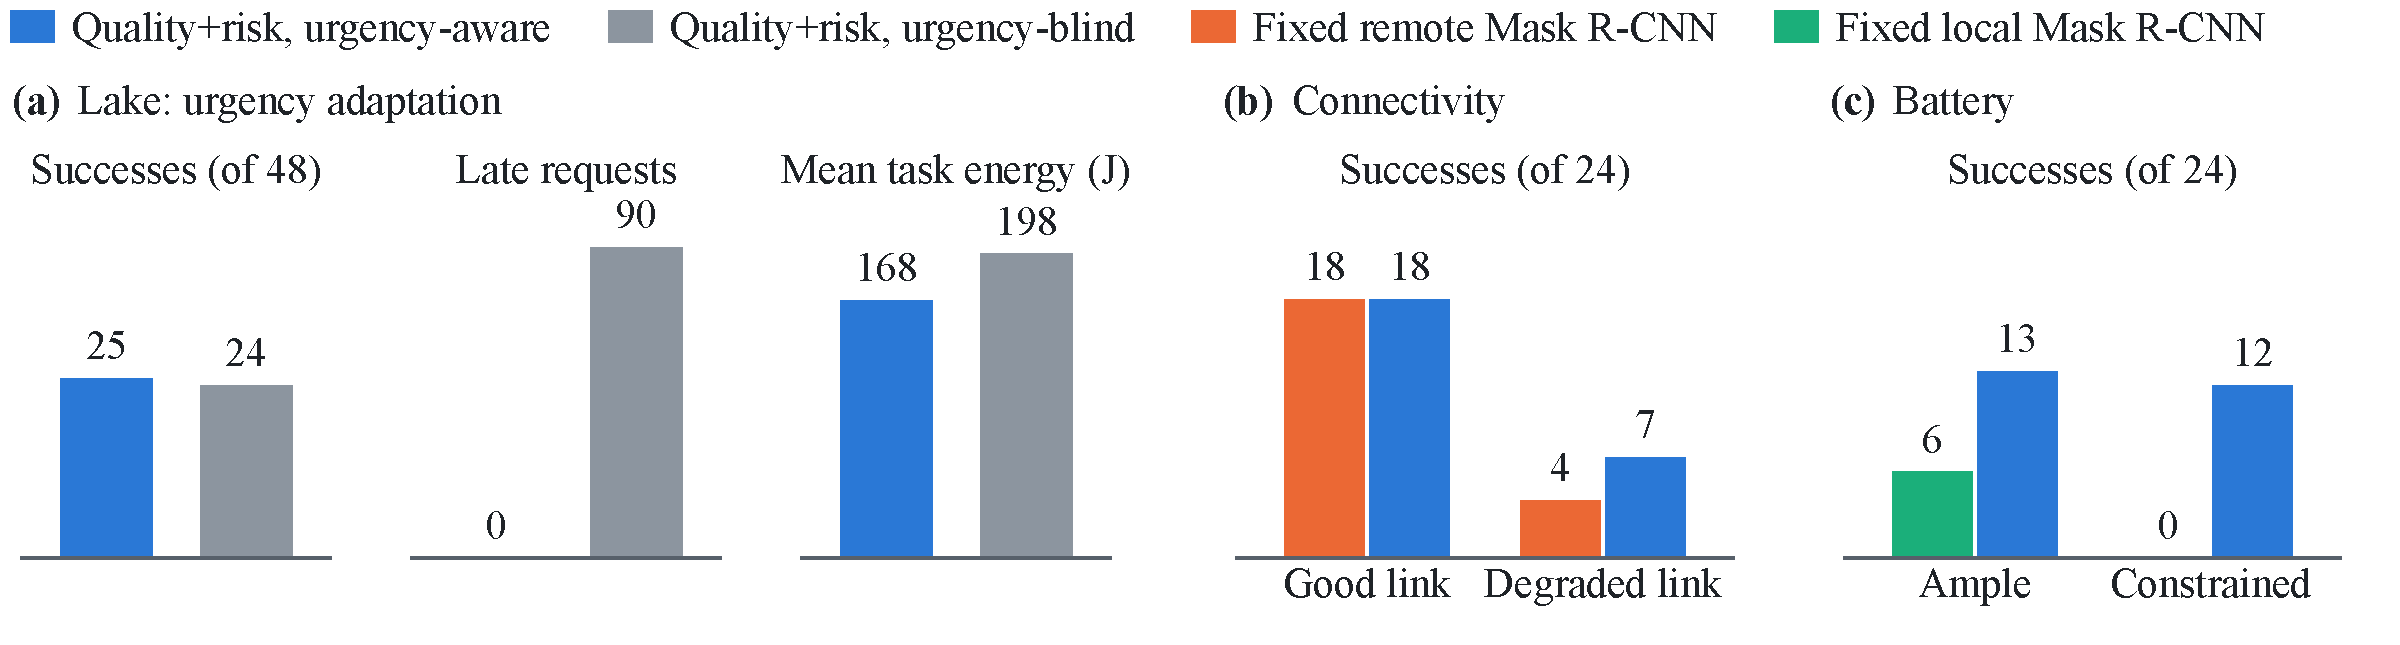
\includegraphics[width=\textwidth]{fig5}
  \caption{Runtime adaptation under changing conditions (Lake, dynamic urgency, transfer
    split: 48 conditions per policy). (a)~Urgency-aware versus urgency-blind quality+risk
    routing: mission successes, late perception requests, and mean modeled task energy per
    run excluding flight energy, each on its own scale. (b)~Successes under good and
    degraded links (24 conditions each). (c)~Successes with ample and constrained battery
    (24 conditions each; constrained starts at the 20\% reserve plus the 42\,s flight
    allocation plus 250\,J for task work). Energy and remote service follow declared models,
    not hardware measurements.}
  \Description{Panel a: urgency-aware routing succeeds in 25 of 48 conditions versus 24 for
    the urgency-blind variant, with 0 versus 90 late requests and 168 versus 198 joules of
    mean task energy. Panel b: fixed remote Mask R-CNN succeeds in 18 of 24 good-link
    conditions and 4 of 24 degraded ones; urgency-aware quality+risk routing succeeds in 18
    and 7. Panel c: fixed local Mask R-CNN succeeds in 6 of 24 conditions with ample battery
    and 0 of 24 when constrained; urgency-aware quality+risk routing succeeds in 13 and 12.}
  \label{fig:runtime-adaptation}
\end{figure*}

\begin{figure*}[t]
  \centering
  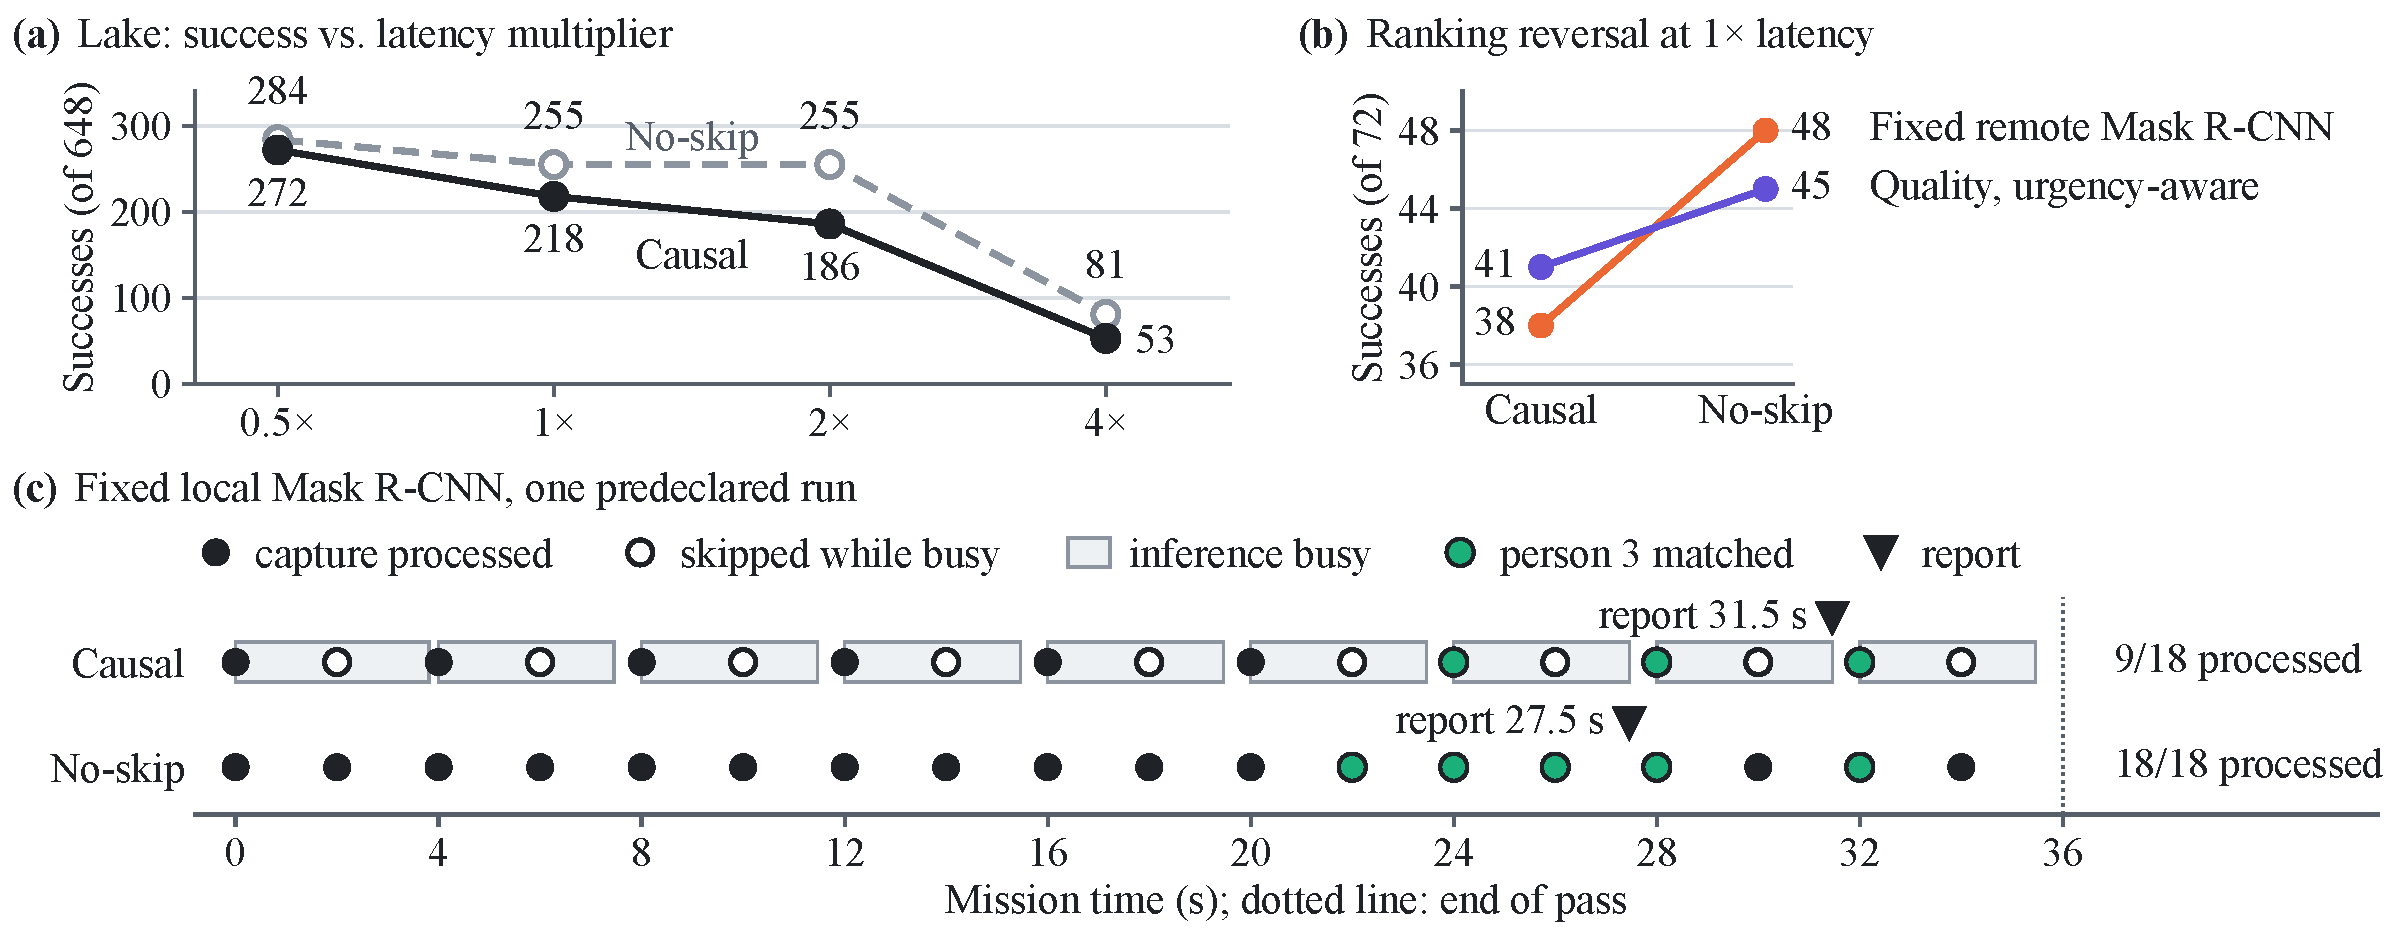
\includegraphics[width=\textwidth]{fig6}
  \caption{Causal execution and observation availability (Lake, dynamic urgency;
    72 conditions $\times$ 9 policies = 648 matched runs per latency setting). (a)~Mission
    successes when inference blocks later captures (causal) versus a no-skip ablation that
    processes every capture as if computation never blocked. The multiplier scales
    inference/service latency and associated local compute energy. Across all four settings,
    only one matched run (at 2$\times$) succeeds
    causally but fails without skipping. (b)~At 1$\times$ latency, ignoring blocking
    reverses the ranking of urgency-aware quality routing and fixed remote Mask R-CNN
    (72 conditions each). (c)~One predeclared run (no urgency change, good link, ample
    battery): local Mask R-CNN takes 3.46\,s per call (3.81\,s for the first) against a 2\,s
    capture interval, so
    causal execution skips every other capture and its first confirmed report arrives 4\,s
    later than under no-skip. Persons~1 and~2 are never matched by this model, so the mission
    fails under both protocols.}
  \Description{Panel a: successes out of 648 at latency multipliers 0.5, 1, 2 and 4 are
    272, 218, 186 and 53 under causal execution and 284, 255, 255 and 81 under the no-skip
    ablation. Panel b: two lines cross; urgency-aware quality routing leads fixed remote
    Mask R-CNN 41 to 38 under causal execution but trails it 45 to 48 under no-skip.
    Panel c: a timeline of 18 captures; causal execution processes 9 and skips 9 while the
    detector is busy, and its report arrives at 31.5 s instead of 27.5 s.}
  \label{fig:causal-execution}
\end{figure*}

\begin{figure*}[t]
  \centering
  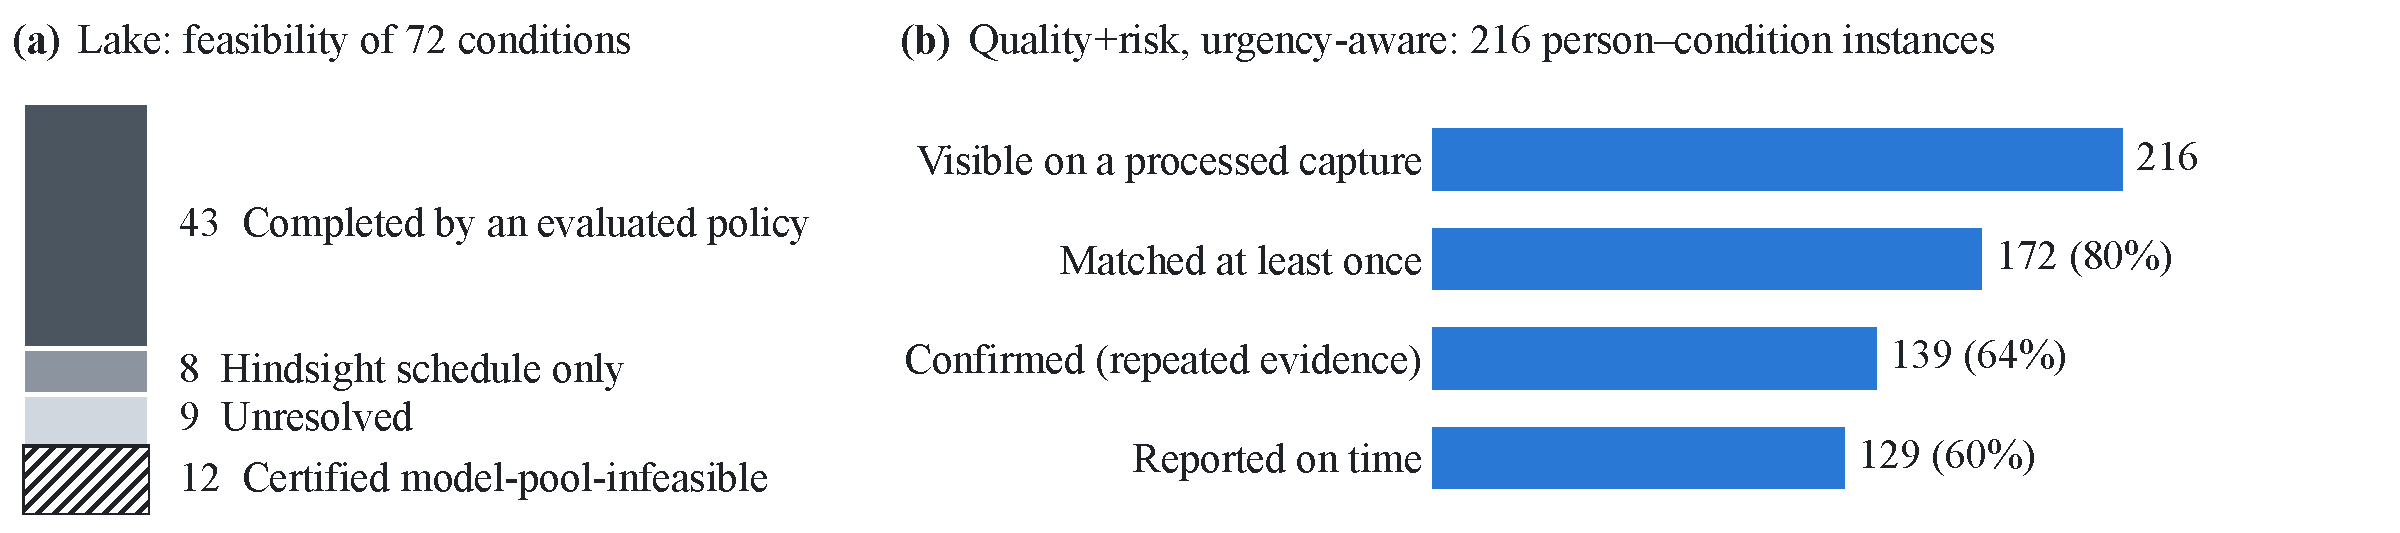
\includegraphics[width=\textwidth]{fig7}
  \caption{Mission feasibility and evidence diagnostics (Lake, dynamic urgency,
    72 conditions). (a)~Four mutually exclusive classes: completed by at least one of the
    nine evaluated policies; completed only by an execution-constrained hindsight schedule
    (an evaluator-only search that uses ground truth and is not a policy, replayed through
    the unchanged runtime); unresolved, where no successful schedule was found but the
    search is not exhaustive; and certified infeasible for the model pool, where even the union
    of all models' matches on every capture, at zero latency, cannot meet the contract. No condition
    is physically infeasible. (b)~Evidence accumulation for urgency-aware quality+risk
    routing over 216 person--condition instances (72 conditions $\times$ 3 focal people);
    percentages are of 216.}
  \Description{Panel a: a segmented bar of 72 conditions with 43 completed by an evaluated
    policy, 8 completed only by a hindsight schedule, 9 unresolved and 12 certified
    infeasible for the model pool. Panel b: of 216 person-condition instances, all 216 are
    visible on a processed capture, 172 are matched at least once, 139 are confirmed by
    repeated evidence and 129 are reported on time.}
  \label{fig:feasibility-evidence}
\end{figure*}
